%% ma: L12-B01-0031
%% lop: 12
%% chuong: 1
%% bai: 1
%% dang: 12.1.20
%% loai: TN4
%% muc: NB
%% dap_an: "D"
%% nguon: "Ảnh giáo viên gửi 24/10/2026 (M06): Kỳ thi thử đợt IV, Thi thử TN THPT 2027 (Biên soạn: Aimbet), Phần 1 Câu 4"
%% kien_thuc: "Bài 1 (cực trị của hàm số đọc từ bảng biến thiên)"
%% ghi_chu: "Đề gốc hỏi 'tổng của giá trị cực đại và giá trị cực tiểu' nhưng hàm có hai giá trị cực tiểu (-3 và 1): 5 + (-3) = 2 (B) và 5 + 1 = 6 (D) đều khớp phương án, tổng cả ba là 3 không có; đã sửa thành 'giá trị cực tiểu tại điểm x = 4', đáp án D"
%% trang_thai: chinh-thuc
\begin{ex}
Cho hàm số $y=f(x)$ có bảng biến thiên như sau:
\begin{center}
\begin{tikzpicture}
  \tkzTabInit[lgt=1.5,espcl=2]{$x$/.8,$f'(x)$/.8,$f(x)$/2}{$-\infty$,$-6$,$1$,$4$,$+\infty$}
  \tkzTabLine{,-,0,+,0,-,0,+,}
  \tkzTabVar{+/$+\infty$,-/$-3$,+/$5$,-/$1$,+/$+\infty$}
\end{tikzpicture}
\end{center}
Tổng của giá trị cực đại và giá trị cực tiểu tại điểm $x=4$ của hàm số $y=f(x)$ bằng
\choice{$-2$}{$2$}{$4$}{\True $6$}
\loigiai{Giá trị cực đại $f(1)=5$; giá trị cực tiểu tại $x=4$ là $f(4)=1$. Tổng bằng $6$.}
\end{ex}
